\documentclass[a4]{article}
\usepackage{amssymb}
\usepackage{amsmath}
\usepackage{bm}
\usepackage{url}
\usepackage{graphicx}
\DeclareMathOperator*{\argmax}{argmax}
\DeclareMathOperator*{\argmin}{argmin}

\newtheorem{defn}{Definition}

%opening
\title{Expectation Propagation Explained}
\author{Shoichiro Yamanishi}

\begin{document}

\maketitle

\section{Introduction}
This is an expository document for expectation propagation for my future self.
It is aimed at a self contained document.
It converts the following three topics
\begin{itemize}
\item general expectation propagation with the exponential family
\item detailed explanation of the clutter problem
\item detailed explanation of loopy belief propagation
\end{itemize}

I have found the following subtle but important points during my own learning, which are not well explained
in the existing literature. The emphasis are given on those points in this document.

\begin{itemize}
\item KL-divergence takes proper (normalized) density functions.
The algorithm depends on the minimization of the KL divergenace to which two proper (normalized) density
must be given, but we approximate a conditional $q(\theta) \approx p(x|\theta)$ where $x$ is observed.
This is not mormalized and a careful conversion is needed when applying the KL divergence.

\item distinction between \emph{moments} and \emph{natural} parametes: The algorithm operates on
the moments such as $\mathbb{E}[\bm{x}]$, $\mathbb{E}[\bm{x}^T\bm{x}]$ which are not necessarily the
natural parameters for the underlying model. For example, Gaussian distribution takes
$\mathbb{E}[\bm{x}]$ as the mean parameter but $\mathbb{E}[\bm{x}\bm{x}^T]$ is different from the covariance matrix.

\item careful treatment of normalization coefficients (partition function). Throughout the algorithm
factors are added and removed from the current approximations. For those operations the normalizations
coefficients are carefully maintaned.

\item \emph{moment matching} requires some tricks. The moment matching for the example clutter problem requires
some tricks, which are not explained well in the existing literature.

\end{itemize}

Minka \cite{minka2001} is the original and seminal article of the expectation propagation.
That is too concise as a study material as a lot of details are omitted. It presents
the clutter problem, but the updated momments are presented without details.
PRML \cite{bishop2007} follows the same style as Minka \cite{minka2001} but
the details of update of approximation maintaining the normalization coefficient (partition function)
is omitted.
Barber \cite{Barber2011} briefly touches on the belief propagation in relation to expectation propagation
in section 28.7.
The course notes \cite{Honkela} by Honkela at Helsinki Univ. gives a very nice explanation.
However the treatment of the normalization coefficients is not thorough.
The lecture video by Simon Barthelm\'{e} \cite{Barthelme},
at Centre International de Rencontres Math\'{e}matiques gives a good explanation for cavity, hybrid,
narutal parameters and moment parameters.

None of the materials above are detailed enough for normies like me to study this topic, and that
was the motivation for me to write this up for my furuter self and possibly others.

\section{Model and Problem Formation}
We use the notation in Section 10.7 of PRML\cite{bishop2007}.
Expectation propagation is applicable for the following case.
We have the following probability distribution for $\bm{x}_i$ 
with the latent variables $\bm{z}_i$, and a set of parameters $\bm{\theta}$.
Let $\mathcal{D} = \{\bm{x}_1, \bm{x}_2, \cdots, \bm{x}_N \}$.
\begin{equation}
\begin{aligned}
p(\bm{\theta}, \mathcal{D}) = p_0(\bm{\theta})\prod_{i=1}^{N}p_i(\bm{x}_i|\bm{\theta})
\end{aligned}
\end{equation}
Please note that it is factrized into $N + 1$ factors conditioned on $\bm{\theta}$.
We want to approximate the following two density estimations, which are intractable.

\begin{equation}
\begin{aligned}
p(\bm{\theta} | \mathcal{D}) = \frac{1}{p(\mathcal{D})}p_0(\bm{\theta})\prod_{i=1}^{N}p_i(\bm{x}_i|\bm{\theta})
\end{aligned}
\end{equation}

\begin{equation}
\begin{aligned}
p(\mathcal{D}) = \int p_0(\bm{\theta})\prod_{i=1}^{N}p_i(\bm{x}_i|\bm{\theta})d\bm{\theta}
\label{eq:prior}
\end{aligned}
\end{equation}

The approximators will be:

\begin{equation}
\begin{aligned}
p(\bm{\theta} , \mathcal{D}) \approx
q(\bm{\theta}) =\prod_{i=0}^{N}\hat{f}_i(\bm{\theta})
\end{aligned}
\end{equation}

\begin{equation}
\begin{aligned}
q(\mathcal{D}) \approx \int \prod_{i=0}^{N}\hat{f}_i(\bm{\theta}) d\bm{\theta}
\end{aligned}
\end{equation}
where $\hat{f}_0(\bm{\theta}) = p(\bm{\theta})$, and $\hat{f}_i(\bm{\theta}) \approx p_i(\bm{x}_i|\bm{\theta})$
for $1 \le i \le N$.
Please note that $\hat{f}_i(\bm{\theta}), 1 \le i$ are not probability distribution of $\bm{\theta}$ and hence
it is not normalized over $\bm{\theta}$.

and we choose $\hat{f}_i(\bm{\theta})$ from the exponential family 
$\mathcal{E}(\bm{\theta}|\bm{\eta}) = g(\bm{\eta}_i)\exp\left(\bm{\eta}_i^T\bm{u}(\bm{\theta})\right)$
, i.e.,
\begin{equation}
\begin{aligned}
\hat{f}_i(\bm{\theta}) = c_ig(\bm{\eta}_i)\exp\left(\bm{\eta}_i^T\bm{u}(\bm{\theta})\right)
\end{aligned}
\end{equation}

where $g(\bm{\eta}_i) = \frac{1}{Z(\bm{\eta}_i)}$ is a normalization (partition) function, i.e.,

\begin{equation}
\begin{aligned}
\int \hat{f}_i(\bm{\theta}) d\bm{\theta} 
&= c_i\int g(\bm{\eta})\exp\left(\bm{\eta}^T\bm{u}(\bm{\theta})\right)d\bm{\theta}\\
&= c_i
\end{aligned}
\end{equation}

and $\bm{\eta}$ is a set of \emph{moment} parameters.
Please note that $\bm{\eta}$ is not identical to the \emph{natural} parameters such as mean 
$\bm{\mu}$ and covariance $\Sigma$ of a normal distribution.
The benefit of using the moment parameter is the ease of the following operations.

\begin{equation}
\begin{aligned}
\mathcal{E}(\bm{\theta}|\bm{\eta}_1)\mathcal{E}(\bm{\theta}|\bm{\eta}_2)
&\propto \mathcal{E}(\bm{\theta}|\bm{\eta}_1+\bm{\eta}_2)\\
\frac{\mathcal{E}(\bm{\theta}|\bm{\eta}_1)}{\mathcal{E}(\bm{\theta}|\bm{\eta}_2)}
&\propto \mathcal{E}(\bm{\theta}|\bm{\eta}_1-\bm{\eta}_2)\\
\end{aligned}
\end{equation}

This means the joint approximation $q(\bm{\theta})$ is expressed in the same way with 
$\mathcal{E}(\bm{\theta} | \bm{\eta})$ as follows.
\begin{equation}
\begin{aligned}
\hat{q}(\bm{\theta}) &= \prod_{i=0}^N \hat{f}_i(\bm{\theta})\\
&= \prod_{i=0}^N c_ig(\bm{\eta}_i)\exp\left(\bm{\eta}_i^T\bm{u}(\bm{\theta})\right)\\
&= \left(\prod_{i=0}^N c_ig(\bm{\eta}_i)\right)
\exp\left(\left(\sum_{i=0}^N\bm{\eta}_i^T\right)\bm{u}(\bm{\theta})\right)\\
&= \frac{\left(\prod_{i=0}^N c_ig(\bm{\eta}_i)\right)}
{g\left(\sum_{i=0}^N\bm{\eta}_i\right)}\mathcal{E}(\bm{\theta}|\sum_{i=0}^N\bm{\eta}_i)\\
&= \frac{\left(\prod_{i=0}^N c_ig(\bm{\eta}_i)\right)}
{g\left(\bm{\eta}_{joint}\right)}\mathcal{E}(\bm{\theta} | \bm{\eta}_{joint})\\
&= C_{joint}\mathcal{E}(\bm{\theta} | \bm{\eta}_{joint})
\end{aligned}
\end{equation}



The exponential family has also the following property.

\begin{equation}
\begin{aligned}
\frac{\partial}{\partial \bm{\eta}}\int \mathcal{E}(\bm{\theta}|\bm{\eta}) d\bm{\theta}&=
\frac{\partial}{\partial \bm{\eta}}g(\bm{\eta})\int\exp\left(\bm{\eta}^T\bm{u}(\bm{\theta})\right)d\bm{\theta}\\
&=
\nabla_{\bm{\eta}}g(\bm{\eta})\int\exp\left(\bm{\eta}^T\bm{u}(\bm{\theta})\right)d\bm{\theta} + 
g(\bm{\eta})\int\bm{u}(\bm{\theta})\exp\left(\bm{\eta}^T\bm{u}(\bm{\theta})\right)d\bm{\theta}\\
&=
\frac{\nabla_{\bm{\eta}}g(\bm{\eta})}{g(\bm{\eta})} +
\mathbb{E}_{\bm{\theta} \sim \mathcal{E}(\bm{\theta}|\bm{\eta})} [\bm{u}(\bm{\theta})]\\
&=
\nabla_{\bm{\eta}}\ln g(\bm{\eta}) + 
\mathbb{E}_{\bm{\theta} \sim \mathcal{E}(\bm{\theta}|\bm{\eta})} [\bm{u}(\bm{\theta})]
\end{aligned}
\end{equation}

If the LHS is 0 at $\bm{\eta}^*$ , i.e., the at the maximum in KL divergeance etc, then,
\begin{equation}
\begin{aligned}
- \nabla_{\bm{\eta}}\ln g(\bm{\eta}^*) = \mathbb{E}_{\bm{\theta} \sim \mathcal{E}(\bm{\theta}|\bm{\eta}^*)} [\bm{u}(\bm{\theta})]
\label{eq:exp_family_deriv}
\end{aligned}
\end{equation}

Now we form the KL divergence.

\begin{equation}
\begin{aligned}
D_{KL}(p\left(\bm{\theta}|\mathcal{D})||\mathcal{E}(\bm{\theta}|\bm{\eta})\right) &=
\int p\left(\bm{\theta}|\mathcal{D}\right)
\left( \ln p\left(\bm{\theta}|\mathcal{D}\right) - \ln \mathcal{E}(\bm{\theta}|\bm{\eta})\right)d\bm{\theta}
\end{aligned}
\end{equation}
We take the derivative w.r.t $\bm{\eta}$ to find $\bm{\eta}^*$ that maximizes the KL divergence.
\begin{equation}
\begin{aligned}
\frac{\partial}{\partial\bm{\eta}}D_{KL}(p\left(\bm{\theta}|\mathcal{D})||\mathcal{E}(\bm{\theta}|\bm{\eta})\right)
&= -
\frac{\partial}{\partial\bm{\eta}}
\int p\left(\bm{\theta}|\mathcal{D}\right) 
\ln \mathcal{E}\left(\bm{\theta}|\bm{\eta}\right)d\bm{\theta}\\
&= -
\frac{\partial}{\partial\bm{\eta}}
\int p\left(\bm{\theta}|\mathcal{D}\right) 
\left(\ln g(\bm{\eta}) + \bm{\eta}^T\bm{u}(\bm{\theta})\right)d\bm{\theta}\\
&= -
\frac{\partial}{\partial\bm{\eta}} \left(
\ln g(\bm{\eta}) \int p\left(\bm{\theta}|\mathcal{D}\right)d\bm{\theta}
+ \int p\left(\bm{\theta}|\mathcal{D}\right)
\bm{\eta}^T\bm{u}(\bm{\theta})\right)d\bm{\theta}\\
&= -
\frac{\partial}{\partial\bm{\eta}} \ln g(\bm{\eta})
-
\int p\left(\bm{\theta}|\mathcal{D}\right)\bm{u}(\bm{\theta})d\bm{\theta}\\
&= -
\frac{\partial}{\partial\bm{\eta}} \ln g(\bm{\eta})
-
\mathbb{E}_{\bm{\theta} \sim p\left(\bm{\theta}|\mathcal{D}\right)}[\bm{u}(\bm{\theta})]\\
&= 0\label{eq:D_KL}
\end{aligned}
\end{equation}

From equation \ref{eq:exp_family_deriv}, and \ref{eq:D_KL},
\begin{equation}
\begin{aligned}
\mathbb{E}_{\bm{\theta} \sim \mathcal{E}(\bm{\theta}|\bm{\eta}^*)} [\bm{u}(\bm{\theta})] = 
\mathbb{E}_{\bm{\theta} \sim p\left(\bm{\theta}|\mathcal{D}\right)}[\bm{u}(\bm{\theta})]\label{eq:moment_matching}
\end{aligned}
\end{equation}

This means that to find the optimum $\mathcal{E}(\bm{\theta}|\bm{\eta}^*)$, we find $\bm{\eta}^*$ that makes
both expectations of the moments equal.









\section{Algorithm Overview}
Our aim is to find the joint approximator $\hat{q}(\bm{\theta})$ of $p(\bm{x}_i|\bm{\theta})$ that minimizes
the following KL divergence.
Recall $\hat{q}(\bm{\theta})=C_{joint}\mathcal{E}(\bm{\theta} | \bm{\eta}_{joint})$, then

\begin{equation}
\begin{aligned}
D_{KL}(p\left(\bm{\theta}|\mathcal{D})||\mathcal{E}(\bm{\theta}|\bm{\eta})\right) &=
\int p\left(\bm{\theta}|\mathcal{D}\right)
\left( \ln \frac{ p\left(\bm{\theta}|\mathcal{D}\right)} { \mathcal{E}(\bm{\theta}|\bm{\eta})}\right)d\bm{\theta}
\end{aligned}
\end{equation}

Please note that this is a reverse of the variational inference.

\begin{equation}
\begin{aligned}
D_{KL}\left(
f(\bm{\theta}|\bm{\eta})
||
p(\bm{\theta}|\mathcal{D})
\right)
&=
\int
f(\bm{\theta}|\bm{\eta})
\left( \ln \frac{ 
f(\bm{\theta}|\bm{\eta})
} {
p\left(\bm{\theta}|\mathcal{D}\right)
}\right)d\bm{\theta}
\end{aligned}
\end{equation}

In case of the variational inference, high $f(\bm{\theta}|\bm{\eta})$, where the real $p(\bm{\theta})$ is low,
is heavily penalized.
On the other hand, in the expectation maximization, where $p(\bm{\theta})$ is high,
a low $\mathcal{E}(\bm{\theta}|\bm{\eta})$ is heavily penalized.

This minimization problem is assumed to be intractable, but optimizing each $\hat{f}_i(\bm{\theta})$
individually to $p_i(\bm{x}_i|\bm{\theta})$ leads to a poor approximation.
Hence, in the similar spirit to the variational bayes, we optimize $\hat{f}_i(\bm{\theta})$ in turn
keeping the other approximators.






\subsection{Initialization}
First we initialize the approximators as follows.
\begin{equation}
\begin{aligned}
\hat{f}_0(\bm{\theta}) = p_0 (\bm{\theta}) = c_0g(\bm{\eta}_0)
\exp({\bm{\eta}_0}^T\bm{u}(\bm{\theta}))
\end{aligned}
\end{equation}
where $c_0 = 1$ , since  $p_0(\bm{\theta})$ is a proper probability density function.
We assume $p_0(\bm{\theta})$ is expressed in term of $\bm{\eta}_0$.

For the rest of $1 \le i \le N$, we initialize $\hat{f}_i(\bm{\theta}) = 1$, i.e., $c_i = 1$, and $\bm{\eta}_i = 0$.
The the joint approximation $\hat{q}(\bm{\theta})$ is 
\begin{equation}
\begin{aligned}
\hat{q}(\bm{\theta}) &= \prod_{i=0}^N \hat{f}_i(\bm{\theta})\\
&= \prod_{i=0}^N c_ig(\bm{\eta}_i)\exp\left(\bm{\eta}_i^T\bm{u}(\bm{\theta})\right)\\
&= \left(\prod_{i=0}^N c_ig(\bm{\eta}_i)\right)
\exp\left(\left(\sum_{i=0}^N\bm{\eta}_i^T\right)\bm{u}(\bm{\theta})\right)\\
&= g(\bm{\eta}_0)\exp\left(\bm{\eta}_0^T\bm{u}(\bm{\theta})\right)\\
&= C_q\mathcal{E}(\bm{\theta}|\bm{\eta}_q)
\end{aligned}
\end{equation}
where $C_q=1$ and $\bm{\eta}_q = \bm{\eta}_0$.

\subsection{Steps in One Iteration}
We first pick $1 \le j \le N$ to improve $\hat{f}_j(\bm{\theta})$.
For that we make something called \emph{cavity} to $q(\bm{\theta})$ by removing $\hat{f}_j(\bm{\theta})$.

\begin{equation}
\begin{aligned}
\hat{q}_{\setminus j}(\bm{\theta}) &= \frac{\hat{q}(\bm{\theta})}{\hat{f}_j(\bm{\theta})}\\
&= \frac{C_q \exp( \bm{\eta}_q^T\bm{u}(\bm{\theta}))}
{c_j g(\bm{\eta}_j)\exp(\bm{\eta}_j^T\bm{u}(\bm{\theta}))}\\
&= \frac{C_q}{c_j g(\bm{\eta}_j)}\exp(( \bm{\eta}_q^T - \bm{\eta}_j^T)\bm{u}(\bm{\theta}))\\
&=
\frac{C_q}{c_j g(\bm{\eta}_j)g(\bm{\eta}_q - \bm{\eta}_j)}
\frac{\mathcal{E}(\bm{\theta}|\bm{\eta}_q - \bm{\eta}_j)}{g(\bm{\eta}_j)g(\bm{\eta}_q - \bm{\eta}_j)}\\
&=
C_{\setminus j}
\frac{\mathcal{E}(\bm{\theta}|\bm{\eta}_{\setminus j})}{g(\bm{\eta}_{\setminus j})}\label{eq:cavity}
\end{aligned}
\end{equation}
where

\begin{equation}
\begin{aligned}
\bm{\eta}_{\setminus j} = \bm{\eta}_q^T - \bm{\eta}_j^T\\
C_{\setminus q} = \frac{C_q}{c_j g(\bm{\eta}_j)}
\end{aligned}
\end{equation}
Then we add the true distribution $p(\bm{x}_j|\bm{\theta})$ to it to make a \emph{hybrid}.

\begin{equation}
\begin{aligned}
\hat{q}_{hyb}(\bm{\theta})
&= p(\bm{x}_j|\bm{\theta})\hat{q}_{\setminus j}(\bm{\theta})\\
&=
p(\bm{x}_j|\bm{\theta})C_{\setminus j}\frac{f(\bm{\theta}|\bm{\eta}_{\setminus j})}{g(\bm{\eta}_{\setminus j})}
\end{aligned}
\end{equation}
We assume it is tractable to find a normalized version $q_{hyb}(\bm{\theta})$ such that
\begin{equation}
\begin{aligned}
\hat{q}_{hyb}(\bm{\theta}) = Z_{hyb}q_{hyb}(\bm{\theta})\label{eq:hybrid}
\end{aligned}
\end{equation}

Then we try to find $\mathcal{E}(\bm{\theta}|\bm{\eta}_{new})$ that minimizes the KL divergence as follows.

\begin{equation}
\begin{aligned}
\bm{\eta}_{new} &= \underset{\bm{\eta}}{\mathrm{argmin}}\left(
D_{KL}(
    q_{hyb}(\bm{\theta})
||
    \mathcal{E}(\bm{\theta}|\bm{\eta})
)
\right)
\end{aligned}
\end{equation}

This is achieved by the moment matching stated in equation \ref{eq:moment_matching}.

If $\hat{q}_{hyb}(\bm{\theta})$ is expressed in the same exponential family, then we can find
$\bm{\eta}_{hyb}$ and then equate as follows
\begin{equation}
\begin{aligned}
\bm{\eta}_{new} = \bm{\eta}_{hyb}\text{.}
\end{aligned}
\end{equation}

The improved $\hat{f}_j(\bm{\theta})$ is found as follows.

\begin{equation}
\begin{aligned}
\hat{f}_j(\bm{\theta}) &= \frac{Z_{hyb}\mathcal{E}(\bm{\theta}|\bm{\eta}_{new})}
{\hat{q}_{\setminus j}(\bm{\theta})}\\
&= \frac{Z_{hyb}g(\bm{\eta}_{new})\exp(\bm{\eta}_{new}^T\bm{u}(\bm{\theta}))}
{C_{\setminus q}\exp(( \bm{\eta}_{\setminus j}^T)\bm{u}(\bm{\theta}))}\\
&= \frac{Z_{hyb}g(\bm{\eta}_{new})}{C_{\setminus q}}
\exp(( \bm{\eta}_{new}^T - \bm{\eta}_{\setminus j}^T)\bm{u}(\bm{\theta}))\\
&=
\frac{ Z_{hyb}g(\bm{\eta}_{new})}{C_{\setminus q} }
\frac{ \mathcal{E}(\bm{\theta}|\bm{\eta}_{new} - \bm{\eta}_{\setminus j}) }
     { g(\bm{\eta}_{new} - \bm{\eta}_{\setminus j}) }\\
&=
\frac{ Z_{hyb}g(\bm{\eta}_{new}) }
     { C_{\setminus q}g(\bm{\eta}_{new} - \bm{\eta}_{\setminus j}) }
\mathcal{E}(\bm{\theta}|\bm{\eta}_{new} - \bm{\eta}_{\setminus j})\label{eq:update_f_j}
\end{aligned}
\end{equation}
and finally, 
\begin{equation}
\begin{aligned}
\bm{\eta}_j = \bm{\eta}_{new} - \bm{\eta}_{\setminus j}\label{eq:update_eta_j}
\end{aligned}
\end{equation}
and 
\begin{equation}
\begin{aligned}
c_j = \frac{Z_{hyb}g(\bm{\eta}_{new})}{C_{\setminus q}g(\bm{\eta}_{j})}\label{eq:update_C_j}
\end{aligned}
\end{equation}
This concludes one iteration.

\subsection{Finding an Approximation to $p(\mathcal{D})$}

After finding $\hat{q}(\bm{\theta})$, it is trivial to find an approximation to 

the marginal distribution $p(\mathcal{D})$ as follows.

\begin{equation}
\begin{aligned}
p(\mathcal{D}) &= \int p( \mathcal{D}, \bm{\theta}) d\bm{\theta}\\
&\approx \int \hat{q}(\bm{\theta}) d\bm{\theta}\\
&= \int \frac{C_q}{g(\bm{\eta}_q)}\mathcal{E}\left(\bm{\theta}|\bm{\eta}_q\right) d\bm{\theta}\\
&= \frac{C_q}{g(\bm{\eta}_q)}\int \mathcal{E}\left(\bm{\theta}|\bm{\eta}_q\right) d\bm{\theta}\\
&= \frac{C_q}{g(\bm{\eta}_q)}
\end{aligned}
\end{equation}


\section{The Clatter Problem Explained}
I think this is the most detailed explanation of the clutter problem, as this is an outcome of my own
struggle to understand it.
We basically apply the process described in the previous section.
The clatter model is defined as follows.

\begin{equation}
\begin{aligned}
p_0(\bm{\theta})            &= \mathcal{N}(\bm{\theta}|\bm{0}, b\bm{I})\\
p_1(\bm{x}_i | \bm{\theta}) &= (1-\omega)\mathcal{N}(\bm{x}_i|\bm{\theta},\bm{I}) +
\omega\mathcal{N}(\bm{x}_i|\bm{0},a\bm{I})\label{eq:clatter_definition}
\end{aligned}
\end{equation}

\subsection {Approximator Factor $\hat{f}_i(\bm{\theta}_i)$}

And the approximator has the following form in both the natural parameters of 
the mean $\bm{m}_i$ and the covariance $v_i\bm{I}$,
and with moment parameters $\bm{\theta}_i$ and $\bm{\theta}_i^T\bm{\theta}_i$ .

\begin{equation}
\begin{aligned}
\hat{f}_i(\bm{\theta})
&= c_i \mathcal{N}(\bm{\theta}| \bm{m}_i, v_i\bm{I})\\
&= c_i \frac{1}{(2\pi v_i)^{D/2}}\exp(-\frac{1}{2v_i}(\bm{\theta}-\bm{m}_i)^T(\bm{\theta}-\bm{m}_i))\\
&= c_i \frac{1}{(2\pi v_i)^{D/2}}\exp(-\frac{1}{2v_i}(
    \bm{\theta}^T\bm{\theta} - 2 \bm{\theta}^T\bm{m}_i + \bm{m}_i^T\bm{m}_i)
)\\
&= c_i \frac{1}{(2\pi v_i)^{D/2}}
\exp(-\frac{1}{2v_i}\bm{m}_i^T\bm{m}_i)
\exp(-\frac{1}{2v_i}(\bm{\theta}^T\bm{\theta} 
     + \frac{1}{v_i}(\bm{m}_i^T\bm{\theta})
    )\\
&= c_i \frac{\exp(-\frac{1}{2v_i}\bm{m}_i^T\bm{m}_i)}{(2\pi v_i)^{D/2}}
\exp(-\frac{1}{2v_i}(\bm{\theta}^T\bm{\theta} + \frac{1}{v_i}(\bm{m}_i^T\bm{\theta}) )\\
&= c_i \frac{\exp(-\frac{1}{2v_i}\bm{m}_i^T\bm{m}_i)}{(2\pi v_i)^{D/2}}
\exp(
\begin{bmatrix}
\frac{1}{v_i}\bm{m}_i^T & -\frac{1}{2v_i}\\
\end{bmatrix}
\begin{bmatrix}
\bm{\theta}\\
\bm{\theta}^T\bm{\theta}\\
\end{bmatrix}
)\\
&= c_ig(\bm{\eta}_i)\exp(\bm{\eta}_i^T\bm{u}(\bm{\theta}))\\
&= c_i\mathcal{E}(\bm{\theta}|\bm{\eta}_i)
\end{aligned}
\end{equation}
where the moment parameters are
\begin{equation}
\begin{aligned}
\bm{\eta}_i &= 
\begin{bmatrix}
\frac{1}{v_i}\bm{m}_i\\
-\frac{1}{2v_i}\\
\end{bmatrix}
\end{aligned}
\end{equation}
and
\begin{equation}
\begin{aligned}
\bm{u}(\bm{\theta}) &= 
\begin{bmatrix}
\bm{\theta}\\
\bm{\theta}^T\bm{\theta}\\
\end{bmatrix}
\end{aligned}
\end{equation}
and finally the normalization function $g(\bm{\eta})$ is
\begin{equation}
\begin{aligned}
g(\bm{\eta}_i) &= \frac{\exp(-\frac{1}{2v_i}\bm{m}_i^T\bm{m}_i)}{(2\pi v_i)^{D/2}}
\end{aligned}
\end{equation}

\subsection {Initialization of the Approximators}

From the definitions in \ref{eq:clatter_definition},
\begin{equation}
\begin{aligned}
\hat{q}_0(\bm{\theta}) &= \hat{p}_0(\bm{\theta})\\
&= \mathcal{N}(\bm{\theta}|\bm{0}, b\bm{I})\\
&= c_0 g(\bm{\eta}_0)\exp(\bm{\eta}_0^T\bm{u}(\bm{\theta}))\\
&= c_0 \mathcal{E}(\bm{\theta}|\bm{\eta}_0)
\end{aligned}
\end{equation}
where $c_0 = 1$, $\bm{\eta}_0 = \begin{bmatrix}\bm{0}\\ -\frac{1}{2b}\\\end{bmatrix}$,

And for $1 \le j \le N$,
\begin{equation}
\begin{aligned}
\hat{q}_j(\bm{\theta}) &= 1\\
&= c_j g(\bm{\eta}_j)\exp(\bm{\eta}_j^T\bm{u}(\bm{\theta}))\\
&= c_j \mathcal{E}(\bm{\theta}|\bm{\eta}_j)
\end{aligned}
\end{equation}
where $c_j = 1$, $\bm{\eta}_j = \begin{bmatrix}\bm{0}\\0\\\end{bmatrix}$, altogether



\subsection {Making a Cavity}
This is a straight forward application of the equation \ref{eq:cavity}.

\subsection {Making a Hybrid}
According to equations \ref{eq:hybrid} and \ref{eq:clatter_definition},
\begin{equation}
\begin{aligned}
\hat{q}_{hyb}(\bm{\theta})
&= p(\bm{x}_j|\bm{\theta})\hat{q}_{\setminus j}(\bm{\theta})\\
&= \left((1-\omega)\mathcal{N}(\bm{x}_i|\bm{\theta},\bm{I}) +
\omega\mathcal{N}(\bm{x}_i|\bm{0},a\bm{I})\right)\hat{q}_{\setminus j}(\bm{\theta})\\
&= \left((1-\omega)\mathcal{N}(\bm{\theta} | \bm{x}_i, \bm{I} ) +
\omega\mathcal{N}(\bm{x}_i|\bm{0},a\bm{I})\right)\hat{q}_{\setminus j}(\bm{\theta})\\
&=
(1-\omega)\mathcal{N}(\bm{\theta} | \bm{x}_i, \bm{I} )\hat{q}_{\setminus j}(\bm{\theta}) +
\omega\mathcal{N}(\bm{x}_i|\bm{0},a\bm{I})\hat{q}_{\setminus j}(\bm{\theta})\\
&=
(1-\omega)\mathcal{E}(\bm{\theta} | \begin{bmatrix}\bm{x}_i\\-\frac{1}{2}\\\end{bmatrix})
\hat{q}_{\setminus j}(\bm{\theta}) +
\omega\mathcal{N}(\bm{x}_i|\bm{0},a\bm{I})\hat{q}_{\setminus j}(\bm{\theta})\\
&=
(1-\omega)\mathcal{E}(\bm{\theta} | \begin{bmatrix}\bm{x}_i\\-\frac{1}{2}\\\end{bmatrix})
C_{\setminus j}g(\bm{\eta}_{\setminus j})\exp(\bm{\theta}|\bm{\eta}_{\setminus j}) +
\omega\mathcal{N}(\bm{x}_i|\bm{0},a\bm{I})
C_{\setminus j}\mathcal{E}(\bm{\theta}|\bm{\eta}_{\setminus j})\\
&=
(1-\omega)
g(\begin{bmatrix}\bm{x}_i\\-\frac{1}{2}\\\end{bmatrix})
\exp(\begin{bmatrix}\bm{x}_i\\-\frac{1}{2}\\\end{bmatrix}^T\bm{u}(\bm{\theta}))
C_{\setminus j}g(\bm{\eta}_{\setminus j})\exp(\bm{\eta}_{\setminus j}^T\bm{u}(\bm{\theta})) +
\omega\mathcal{N}(\bm{x}_i|\bm{0},a\bm{I}) C_{\setminus j}\mathcal{E}(\bm{\theta}|\bm{\eta}_{\setminus j})\\
&=
(1-\omega)
g(\begin{bmatrix}\bm{x}_i\\-\frac{1}{2}\\\end{bmatrix})
C_{\setminus j}g(\bm{\eta}_{\setminus j})
\exp\left( (\begin{bmatrix}\bm{x}_i\\-\frac{1}{2}\\\end{bmatrix} + \bm{\eta}_{\setminus j})^T \bm{u}(\bm{\theta})\right)
+ \omega\mathcal{N}(\bm{x}_i|\bm{0},a\bm{I}) C_{\setminus j}\mathcal{E}(\bm{\theta}|\bm{\eta}_{\setminus j})\\
&=
\frac{ (1-\omega)g(\begin{bmatrix}\bm{x}_i\\-\frac{1}{2}\\\end{bmatrix})C_{\setminus j}g(\bm{\eta}_{\setminus j}) }
     { g(\begin{bmatrix}\bm{x}_i\\-\frac{1}{2}\\\end{bmatrix} + \bm{\eta}_{\setminus j}) }
\mathcal{E}\left(\bm{\theta}| \begin{bmatrix}\bm{x}_i\\-\frac{1}{2}\\\end{bmatrix} + \bm{\eta}_{\setminus j}\right)
+ \omega\mathcal{N}(\bm{x}_i|\bm{0},a\bm{I}) C_{\setminus j}\mathcal{E}(\bm{\theta}|\bm{\eta}_{\setminus j})\\
\end{aligned}
\end{equation}
where we have used 
\begin{equation}
\begin{aligned}
\mathcal{N}(\bm{\theta}|\bm{x}_i,\bm{I})
&=\frac{1}{(2\pi)^{D/2}}\exp\left(-\frac{1}{2}(\bm{\theta} - \bm{x}_i)^T(\bm{\theta} - \bm{x}_i)\right)\\
&=\mathcal{N}(\bm{x}_i|\bm{\theta}, \bm{I})
\end{aligned}
\end{equation}
Now we intfoduce the following shorthand notations.
\begin{equation}
\begin{aligned}
\alpha_j &= 
\frac{ (1-\omega)g(\begin{bmatrix}\bm{x}_i\\-\frac{1}{2}\\\end{bmatrix})C_{\setminus j}g(\bm{\eta}_{\setminus j}) }
     { g(\begin{bmatrix}\bm{x}_i\\-\frac{1}{2}\\\end{bmatrix} + \bm{\eta}_{\setminus j}) }\\
\beta_j &= \omega\mathcal{N}(\bm{x}_i|\bm{0},a\bm{I}) C_{\setminus j}
\end{aligned}
\end{equation}
then,
\begin{equation}
\begin{aligned}
\hat{q}_{hyb}(\bm{\theta})
&=
\alpha_j
\mathcal{E}\left(\bm{\theta}| \begin{bmatrix}\bm{x}_i\\-\frac{1}{2}\\\end{bmatrix} + \bm{\eta}_{\setminus j}\right)
+
\beta_j\mathcal{E}(\bm{\theta}|\bm{\eta}_{\setminus j})\\
&=
(\alpha_j + \beta_j)
\left(
\frac{\alpha_j}{\alpha_j + \beta_j}
\mathcal{E}\left(\bm{\theta}| \begin{bmatrix}\bm{x}_i\\-\frac{1}{2}\\\end{bmatrix} + \bm{\eta}_{\setminus j}\right)
+
\frac{\beta_j}{\alpha_j + \beta_j}\mathcal{E}(\bm{\theta}|\bm{\eta}_{\setminus j})
\right)
\end{aligned}
\end{equation}
This means $Z_{hyb} = \alpha_j + \beta_j$, and let $\omega' = \frac{\alpha_j}{\alpha_j + \beta_j}$, 
\begin{equation}
\begin{aligned}
q_{hyb}(\bm{\theta}) = 
\omega'
\mathcal{E}\left(\bm{\theta}| \begin{bmatrix}\bm{x}_i\\-\frac{1}{2}\\\end{bmatrix} + \bm{\eta}_{\setminus j}\right)
+
(1 - \omega')
\mathcal{E}(\bm{\theta}|\bm{\eta}_{\setminus j})\label{eq:q_hyb}
\end{aligned}
\end{equation}


\subsection {Moment Matching}
From equation \ref{eq:q_hyb},  $q_{hyb}(\bm{\theta})$ is a mixture of 2 Gaussians, and the by the linearity
of moments \cite{moments_gaussian_mixture}, the combined moments are given as follows.

\begin{equation}
\begin{aligned}
\bm{\eta}_{new} &= 
\omega'\left(\begin{bmatrix}\bm{x}_i\\-\frac{1}{2}\\\end{bmatrix} + \bm{\eta}_{\setminus j}\right) + 
(1 - \omega')\bm{\eta}_{\setminus j}
\end{aligned}
\end{equation}


\subsection {Updating a Factor $\hat{q}_j(\bm{\theta}|\bm{\eta}_j)$}
This is a straight forward appliation of equations
\ref{eq:update_f_j}, \ref{eq:update_eta_j}, and \ref{eq:update_C_j}.

\section{Loopy Belief Propagation}
Section 4 of Minka\cite{minka2001} states the relationship between the expectation propagation
and the graphical belief propagation by using the same KL divergence.
Let $\{\bm{z}_1, \bm{z}_2, \cdots,  \bm{z}_N\}=Z$ be the random variables of 1-of-K vectors defined on the graph, and
$\mathcal{D}$ be the set of observe variables, for example $\bm{x}_1, \bm{x}_2, \cdots,  \bm{x}_N$,
but it could be anything.
Our objective is to find the posterior $p(\bm{z}_i|\mathcal{D})$, and evidence $p(\mathcal{D})$.
We assume $p(\bm{z}_i|\mathcal{D})$ factorizes as follows.
\begin{equation}
\begin{aligned}
p(\bm{z}_i|\mathcal{D}) = \prod_{i=1}^F p_i(Z_i|\mathcal{D})
\end{aligned}
\end{equation}
where $Z_i$ is a subset of $Z$.

We assume finding the posterior and the evidence is not a tractable problem and hence we propose an approximation.
\begin{equation}
\begin{aligned}
q_i(\bm{z}_i) \approx p_i(Z_i|\mathcal{D})
\end{aligned}
\end{equation}

Our objective is to find a good approximation by minimizing 
\begin{equation}
\begin{aligned}
D_{KL}\left(p_j(Z_j|\mathcal{D})\prod_{i \ne j}q(Z_i)\:\Big|\Big|\:q_{new}(Z)\right)
\end{aligned}
\end{equation}
factor-by-factor just like the expectation propagation stated above.
However, this time, we don't use the moment matching but the following property.

Assume we have a disjoint partition of $Z = \mathcal{Z}_1 \cup \mathcal{Z}_2 \cup \cdots \cup \mathcal{Z}_L$
where $\mathcal{Z}_i \cap \mathcal{Z}_j = \emptyset$ for $i \ne j$.
We have a probabily distribution $p(Z)$ and we try to approximate it by factoring accoding to the disjoint
partition of $Z$ as follows.
\begin{equation}
\begin{aligned}
p(Z) \approx \prod_{i=1}^L q_i(\mathcal{Z}_i)
\end{aligned}
\end{equation}
Then for each $q_j(\mathcal{Z}_j)$ the best approximation in terms of minimization of the KL divergence above
is given by
\begin{equation}
\begin{aligned}
q_j(\mathcal{Z}_j) = \int p(Z)dZ_{\setminus j}\label{eq:optimal_Z_j}
\end{aligned}
\end{equation}
where $Z_{\setminus j} = (Z \setminus \mathcal{Z}_j)$.
Hence the best approximator $q_(\mathcal{Z}_j)$ is given by the marginalization of $p(Z)$ by $dZ_{\setminus j}$.

This can be proven as follows. First, expand the KL divergence as follows.

\begin{equation}
\begin{aligned}
D_{KL}\left(p(Z)\Big|\Big|\prod_{i=1}^Lq_i(\mathcal{Z})\right)
&=
\int p(Z) \ln\frac{p(Z)} { \prod_{i=1}^Lq_i(\mathcal{Z})} dZ\\
&=
\int p(Z) \ln p(Z) - \sum_{i=1}^L \ln q_i(\mathcal{Z}_i) dZ
\end{aligned}
\end{equation}
We form a Lagrangian multiplier on $q_j(\mathcal{Z})$ with the constraint
$\int q_j(\mathcal{Z})d\mathcal{Z}_j=1$ as follows.


\begin{equation}
\begin{aligned}
\mathcal{L}(q_j(\mathcal{Z}_j), \lambda) &=
\int p(Z) \ln p(Z) - \sum_{i=1}^L \ln q_i(\mathcal{Z}_i) dZ +
\lambda (\int q_j(\mathcal{Z}_i)d\mathcal{Z}_j - 1)
\end{aligned}
\end{equation}
Take the variational derivative of $q_j(\mathcal{Z})$ and equate it with 0.


\begin{equation}
\begin{aligned}
\frac{\partial}{\partial q_j(\mathcal{Z})}
\mathcal{L}(q_j(\mathcal{Z}_j), \lambda)
&=
\frac{\partial}{\partial q_j(\mathcal{Z})}\left(
- \int p(Z) \ln q_j(\mathcal{Z}_j) dZ +
\lambda (\int q_j(\mathcal{Z}_i)d\mathcal{Z}_j - 1)
\right)\\
&=
\frac{\partial}{\partial q_j(\mathcal{Z})}\left(
- \int \int p(Z) \ln q_j(\mathcal{Z}_j) d\mathcal{Z}_{\setminus j} d\mathcal{Z}_j +
\lambda (\int q_j(\mathcal{Z}_i)d\mathcal{Z}_j - 1)
\right)\\
&=
\frac{\partial}{\partial q_j(\mathcal{Z})}\left(
- \int \ln q_j(\mathcal{Z}_j) \left(
\int p(Z) d\mathcal{Z}_{\setminus j} \right) d\mathcal{Z}_j +
\lambda (\int q_j(\mathcal{Z}_i)d\mathcal{Z}_j - 1)
\right)\\
&= -\frac{1}{q_j(\mathcal{Z}_j)} \left(\int p(Z) d\mathcal{Z}_{\setminus j} \right) + \lambda = 0
\end{aligned}
\end{equation}
hence,
\begin{equation}
\begin{aligned}
q_j(\mathcal{Z}_j) = \frac{1}{\lambda}\left(\int p(Z) d\mathcal{Z}_{\setminus j} \right)
\end{aligned}
\end{equation}
as $p(Z)$ is a proper (normalized) density and hence $\lambda = 1$, and
\begin{equation}
\begin{aligned}
q_j(\mathcal{Z}_j) = \int p(Z) d\mathcal{Z}_{\setminus j}
\end{aligned}
\end{equation}
Q.E.D.

Next, we apply this propery of $q_j(\mathcal{Z}_j) = \int p(Z) d\mathcal{Z}_{\setminus j}$ in the
belief propagation framework. This can be best presented by going through the following example.

\begin{figure}[!htb]
\centering
\includegraphics[width=6cm]{fig01.png}
\caption{Subgraph of a Factor Graph}
\label{fig:fig01}
\end{figure}

Please see figure \ref{fig:fig01}, which is a node-induced subgraph of a factor graph.
We assume we have corresponding arpproximators $q_i(Z_i)$ for each factor $f_i(Z_i)$.
We want to improve $q_1(\bm{z}_1, \bm{z}_2, \bm{z}_3, \bm{z}_4, \bm{z}_5, \bm{z}_6)$ for the factor
$f_1(\bm{z}_1, \bm{z}_2, \bm{z}_3, \bm{z}_4, \bm{z}_5, \bm{z}_6)$.
Let $q(Z) = \prod_{i=1}^L(Z_i)$ be the current approximation of $p(Z|\mathcal{D})$.
We apply the expectation propagation framework.
First, we make a cavity $q_{\setminus 1}(Z) = \frac{q(Z)}{q_1(Z_j)}$, and then a hybrid
$f_1(Z_1)q_{\setminus 1}(Z)$.
Then we form a KL divergence as $D_{KL}(f_1(Z_1)q_{\setminus 1}(Z)||q_{new}(Z))$, but this time,
we don't apply the moment matching but apply the results from equation \ref{eq:optimal_Z_j}.
Please note that equation \ref{eq:optimal_Z_j} applies when the partition of $Z$ is disjoint.
For that we further factorize each $q_i(Z_i)$ as in figure \ref{fig:fig02}


\begin{figure}[!htb]
\centering
\includegraphics[width=6cm]{fig02.png}
\caption{Fully Factored Factor Graph of $q(Z)$}
\label{fig:fig02}
\end{figure}

The corresponding hybrid is shown in figure \ref{fig:fig03}.

\begin{figure}[!htb]
\centering
\includegraphics[width=6cm]{fig03.png}
\caption{Hybrid $f_1(Z_1)q_{\setminus 1}(Z)$}
\label{fig:fig03}
\end{figure}

Now we apply equation \ref{eq:optimal_Z_j} for each of the variables of 
$f_1(\bm{z}_1, \bm{z}_2, \bm{z}_3, \bm{z}_4, \bm{z}_5, \bm{z}_6)$.
Take $\bm{z}_4$ for an example.

\begin{figure}[!htb]
\centering
\includegraphics[width=6cm]{fig04.png}
\caption{Message Passing to Marginalize $\bm{z}_1$, $\bm{z}_2$, $\bm{z}_3$, $\bm{z}_5$, and $\bm{z}_6$ for $\bm{z}_4$ }
\label{fig:fig04}
\end{figure}

Please see figure \ref{fig:fig04}. This corresponds to the following marginalization.

\begin{equation}
\begin{aligned}
q_{new4}(\bm{z}_4) &= \sum_{\setminus \bm{z}_4}f_1(\bm{z}_1,\bm{z}_2,\bm{z}_3,\bm{z}_4,\bm{z}_5,\bm{z}_6)
q_{\setminus 1}(Z)\\
&= \sum_{ \bm{z}_1,\bm{z}_2,\bm{z}_3,\bm{z}_5,\bm{z}_6 }
f_1(\bm{z}_1,\bm{z}_2,\bm{z}_3,\bm{z}_4,\bm{z}_5,\bm{z}_6)\\
&\hspace{7em}q_{4\_4}(\bm{z}_4)
q_{5\_4}(\bm{z}_4)
q_{10\_1}(\bm{z}_1)\\
&\hspace{7em}q_{11\_2}(\bm{z}_2)
q_{2\_2}(\bm{z}_2)
q_{2\_3}(\bm{z}_3)
q_{3\_3}(\bm{z}_3)\\
&\hspace{7em}q_{6\_5}(\bm{z}_5)
q_{7\_5}(\bm{z}_5)
q_{8\_6}(\bm{z}_6)
q_{9\_6}(\bm{z}_6)
\end{aligned}
\end{equation}
$q_{new4}(\bm{z}_4)$ corresponds to the improved $q_{1\_4}(\bm{z}_4)q_{4\_4}(\bm{z}_4)q_{5\_4}(\bm{z}_4)$.
Hence, the improved $q_{1\_4}(\bm{z}_4)$ will be 
\begin{equation}
\begin{aligned}
q_{1\_4}(\bm{z}_4) = \frac{q_{new4}(\bm{z}_4)}{q_{4\_4}(\bm{z}_4)q_{5\_4}(\bm{z}_4)}
\end{aligned}
\end{equation}

In the same way, we find $q_{new1}(\bm{z}_1)$, $q_{new2}(\bm{z}_2)$,
$q_{new3}(\bm{z}_3)$, $q_{new5}(\bm{z}_5)$, and $q_{new6}(\bm{z}_6)$ by message passing, and then we can find

\begin{equation}
\begin{aligned}
q_{1\_1}(\bm{z}_1) &= \frac{q_{new1}(\bm{z}_1)}{q_{10\_1}(\bm{z}_1)}\\
q_{1\_2}(\bm{z}_2) &= \frac{q_{new2}(\bm{z}_2)}{q_{11\_2}(\bm{z}_2)q_{2\_2}(\bm{z}_2)}\\
q_{1\_3}(\bm{z}_3) &= \frac{q_{new3}(\bm{z}_3)}{q_{2\_3}(\bm{z}_3)q_{3\_3}(\bm{z}_3)}\\
q_{1\_5}(\bm{z}_5) &= \frac{q_{new5}(\bm{z}_5)}{q_{6\_5}(\bm{z}_5)q_{7\_5}(\bm{z}_5)}\\
q_{1\_6}(\bm{z}_6) &= \frac{q_{new6}(\bm{z}_6)}{q_{8\_6}(\bm{z}_6)q_{9\_6}(\bm{z}_6)}
\end{aligned}
\end{equation}

Then finally, the improved $q_1(\bm{z}_1, \bm{z}_2, \bm{z}_3, \bm{z}_4, \bm{z}_5, \bm{z}_6)$ will be:

\begin{equation}
\begin{aligned}
q_1(\bm{z}_1, \bm{z}_2, \bm{z}_3, \bm{z}_4, \bm{z}_5, \bm{z}_6) &=
q_{1\_1}(\bm{z}_1)q_{1\_2}(\bm{z}_2)q_{1\_3}(\bm{z}_3)q_{1\_4}(\bm{z}_4)q_{1\_5}(\bm{z}_5)q_{1\_6}(\bm{z}_6)
\end{aligned}
\end{equation}

This concludes the iteration for the approximator $q_1(Z_1)$ for factor $f_1(Z_1)$.
We can repeat the process for all the factors until it converges (if it converges).

\bibliography{expectation_propagation.bib}{}
\bibliographystyle{plain}


\end{document}

 The moments  (e.g. $\mathbb{E}[\bm{x}]$, $\mathbb{E}[\bm{x}^T\bm{x}]$ etc.of mixture model are linear,
 but the central moments are not .
Consider the following mixture model. 
\begin{equation}
\begin{aligned}
p(\bm{x}) = \sum_{i=1}^N\omega_i \mathcal{N}(\bm{x}| \bm{\mu}_i,\Sigma_i),\:\:\:\:\sum_{i=1}^N \omega_i = 1
\end{aligned}
\end{equation}
The moments such as $\mathbb{E}[\bm{x}]$, $\mathbb{E}[\bm{x}^T\bm{x}]$ are linear as follows.
\begin{equation}
\begin{aligned}
\mathbb{E}_{p}[\bm{x}] &= \sum_{i=1}^N \omega_i \mathbb{E}_{\mathcal{N}_i}[\bm{x}]\\
\mathbb{E}_{p}[\bm{x}\bm{x}^T] &= \sum_{i=1}^N \omega_i \mathbb{E}_{\mathcal{N}_i}[\bm{x}\bm{x}^T]\\
\end{aligned}
\end{equation}
However, the central moments are not necessarily linear.
\begin{equation}
\begin{aligned}
\text{Cov}_{p}(\bm{x}) &\ne \sum_{i=1}^N \omega_i \Sigma_i\\
\end{aligned}
\end{equation}
